%----------------------------------------------------------------------------
\chapter{A rendszer architektúrája}
%----------------------------------------------------------------------------

Az alkalmazás architektúrája három nagyobb komponensből áll. Mindhárom egy különálló szerver, amelyek egy összefüggő gráfként képesek kommunikálni egymással (\ref{abra:architecture}).

\begin{figure}[!h]
	\centering
	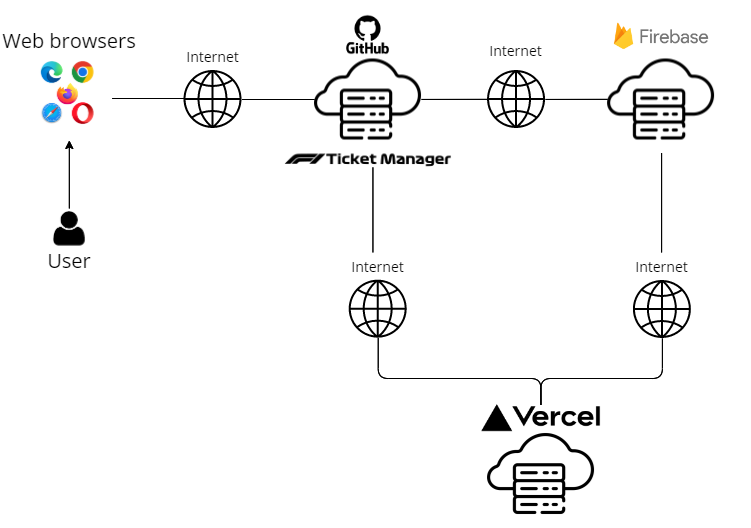
\includegraphics[scale=0.7]{images/architecture}
	\caption{Rendszer architekúra}
	\label{abra:architecture}
\end{figure}

Az rendszer fő komponense a weboldalt üzemeltető szerver, a \textbf{GitHub Pages}. Ez felel az oldal rendereléséért és valós időben elérhetőségéről. Erre azért van lehetőség, mivel a forráskód megtalálható a GitHub-on, amelyet összekötöttem a GitHub Pages-el. A deployment fázis során a GitHub egy optimalizált kódot generál és azt hosztolja \cite{Deploy}.

A második komponens a \textbf{Google Firebase} CDN alapú felhőalapú szolgáltató. Segítségével meg lehet valósítani felhasználók autentikációját, adatok tárolását egy NoSQL adatbázis-kezelő rendszerben és még sok mást. Azért ezeket emeltem ki, mivel ezek a funkcionalitások játszanak szerepet a rendszerben. A weboldal folyamatosan kommunikál a Google Firebase-el, hogy valós időben és hatékonyan tudja kiszolgálni a felhasználókat. Az \textbf{F1 Ticket Manager} egyik központi eleme a jegyek kezelése, amely során titkosítási algoritmusok futnak a felhasználók adatainak biztonsága érdekében. Mivel ezeket az algoritmusokat nem lehetséges, hogy a Google Firebase ingyenes verziójával igénybe vegyem, ezért szükségem volt egy másik backend szerverre is, ahol el tudom végezni ezeket a műveleteket.

A harmadik és egyben utolsó komponens a \textbf{Vercel} felhőalapú szolgáltató, amelyen fut egy NodeJs szerver, amelyet én fejlesztettem. Ennek a szervernek a API-jai felelnek a titkosítási folyamatokért. Mivel az adatok csak a {Google Firestore}-ban vannak tárolva, ezért elengedhetetlen, hogy kommunikáljon vele. 

\section {GitHub frontend architektúra} \label{frontend}

A rendszer frontendjét szolgáló komponens, amelyet a GitHub Pages hosztol, egy \textbf{create-react-app} alkalmazás. Ez egy olyan \textbf{npm} (\ref{abra:npmLogo}) JavaScript futási környezet csomagkezelője \cite{WikiNpm} által forgalmazott projekt sablon, amely tartalmazza az alapvető konfigurációkat és fájlokat, amelyek szükségesek egy \textbf{React} alkalmazás készítéséhez.

\begin{figure}[!h]
	\centering
	
\includegraphics[scale=0.2]{images/npmLogo}
	\caption{Az npm csomagkezelő}
	\label{abra:npmLogo}
\end{figure}

Az F1TM frontend kódbázisának gyökérkönyvtára az \textit{src} mappa (\ref{abra:srcFolderStructure}), amely tartalmazza az alkalmazás komponenseit, oldalait, a többi szerver végpontjaira kapcsolódó függvényeket és a React \textbf{Redux} kezelésére használt kódokat.

\begin{figure}[!h]
	\centering
	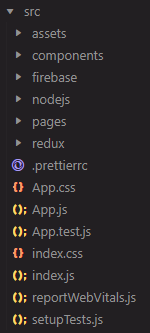
\includegraphics[scale=0.6]{images/srcFolderStructure}
	\caption{Az src mappa struktúrája}
	\label{abra:srcFolderStructure}
\end{figure}

A mappa struktúrába rendezett komponensek (\ref{abra:components}) áttekinthetőbbé teszik a rendszert. Az adott funkcióhoz tartozó összes fájl vagy modul egy helyen vannak, így könnyen megtalálhatóak és karbantarthatóak. Ez különösen hasznos, ha több fejlesztő dolgozik ugyanazon a rendszeren, vagy ha idővel vizsgálni vagy módosítani kell a komponenseket.

Az alaposan megszervezett struktúra lehetővé teszi a komponensek könnyű újrafelhasználását. Ez jelentősen csökkentheti a fejlesztési időt és erőforrásokat, mivel nem kell mindent újra implementálni vagy átírni.

Továbbá egy új funkció bevezetésénél nagyon megkönnyíti a mapparendszer, hogy könnyen megtaláljam a megfelelő helyét az új fájloknak. Az új funkciót egy új komponensként hozzáadhatjuk a megfelelő mappába anélkül, hogy át kellene írni vagy megváltoztatni a meglévő komponenseket. Ez tisztább és kevésbé összezavaró kódbázist eredményez, és minimalizálja a mellékhatásokat vagy a hibák kockázatát.

\begin{figure}[!h]
	\centering
	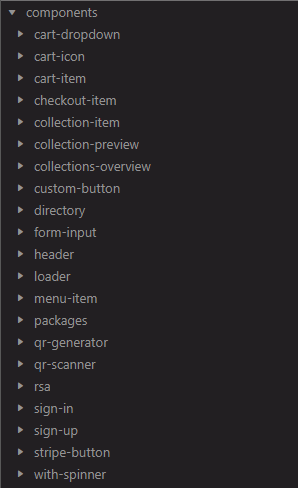
\includegraphics[scale=0.6]{images/components}
	\caption{Komponensek}
	\label{abra:components}
\end{figure}

A \textbf{Vercel} szerverrel való kommunikációra az \textbf{axios} csomagot használtam. Ennek segítségével tudom kezelni a hálózaton történő HTTP kéréseket, amelyekhez hozzátartozik az url, body és egyéb paraméterek megadása.

\section {Google Firebase backend architektúra} \label{firebase}

A \textbf{Google Firebase} olyan platform, amely lehetővé teszi a fejlesztők számára, hogy könnyedén építsenek és üzemeltessenek felhőalapú alkalmazásokat. A Firebase architektúrája több szolgáltatásból áll, amelyek együttműködnek, hogy biztosítsák a fejlesztők számára a skálázhatóságot, megbízhatóságot és az alkalmazások széleskörű funkcióit (\ref{abra:firebaseConsole}).

A Google Firebase funkcionalitásainak elérésére léteznek direkt JavaScript alapú keretrendszerekre könyvtárcsomagok. ReactJs-re a \textit{firebase} és annak almoduljai a \textit{/storage}, \textit{/compat/app}, \textit{/compat/auth} vagy a \textit{/compat/firestore}, míg NodeJS-ben a \textit{firebase-admin}. Ezekben a modulokban implementálva minden kérés a Firebase felé és a visszakapott adatok deszerializálása. Például a \textbf{storage} modullal lehetséges a Cloud Storage kezelése és az \textbf{auth}-al a felhasználók bejelentkeztetése és az adataik kezelése.

\begin{figure}[!h]
	\centering
	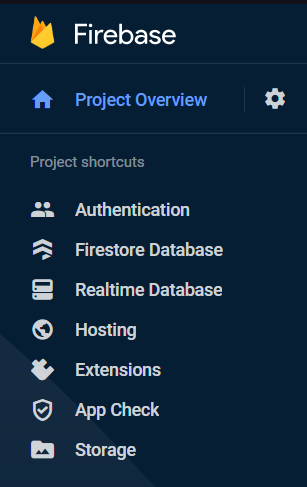
\includegraphics[scale=0.6]{images/firebaseConsole}
	\caption{Firebase Console}
	\label{abra:firebaseConsole}
\end{figure}
\pagebreak

\subsection {Firebase Authentication}

A rendszeremben az egyik központi szerepet játszó szolgáltatás a \textbf{Firebase Authentication}. Ennek segítségével a felhasználók regisztrálhatnak, bejelentkezhetnek és hitelesíthetik magukat az alkalmazásban. Ez a szolgáltatás támogatja az email-alapú, és közösségi média alapú hitelesítési módokat is, és lehetővé teszi a felhasználói adatok kezelését. Az F1 Ticket Managerben lehetőség van regisztrálni email cím, Google vagy Facebook fiók segítségével (\ref{abra:loginMethods}). Amennyiben saját email fiókkal történik a regisztráció, szükség van annak vissza igazolására, amely a megadott fiókra érkező levélben megadott linkkel lehetséges.

\begin{figure}[!h]
	\centering
	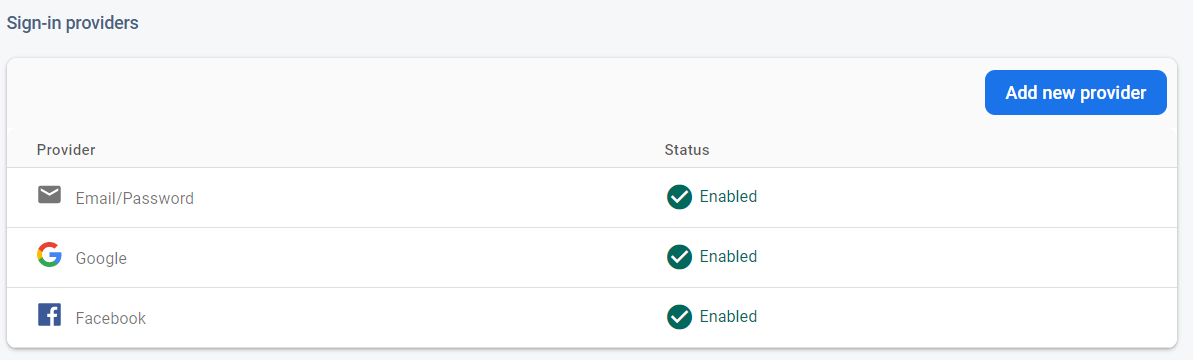
\includegraphics[scale=0.4]{images/loginMethods}
	\caption{Autentikációs módok}
	\label{abra:loginMethods}
\end{figure}

A \ref{firebase} fejezetben is említett \textit{/compat/auth} modul által lehetőségem van a rendszer bármely pontján elérni az aktuálisan bejelentkezett felhasználó adatait a \textit{firebase.currentUser}-en keresztül.

\subsection {Cloud Firestore}

A második, általam leghasználtabb, funkcionalitás a \textbf{Cloud Firestore}. A Firestore egy dokumentum-orientált adatbázis, amely skálázhatóbb és rugalmasabb lehetőségeket kínál adatok tárolására és lekérdezésére. Firestore használatakor a fejlesztők strukturált gyűjteményeket és dokumentumokat hozhatnak létre, és lehetőségük van komplex lekérdezések végrehajtására és az adatok szűrésére. Ilyen dokumentumokban tárolom a felhasználói adatokat, amelyek nagyrésze meg is jelenik a felületen, a pályák és jegyek adatait, valamint a rendeléseket (\ref{abra:firestoreStructure}). A pályaadatokat egy JSON fájlban gyűjtöttem össze és abba lehetséges a módosításuk is, majd egy általam írt kód segítségével ebből a JSON adatcsomagból létrehozok egy többrétegű dokumentumrendszert a Firestoreban.

\begin{figure}[!h]
	\centering
	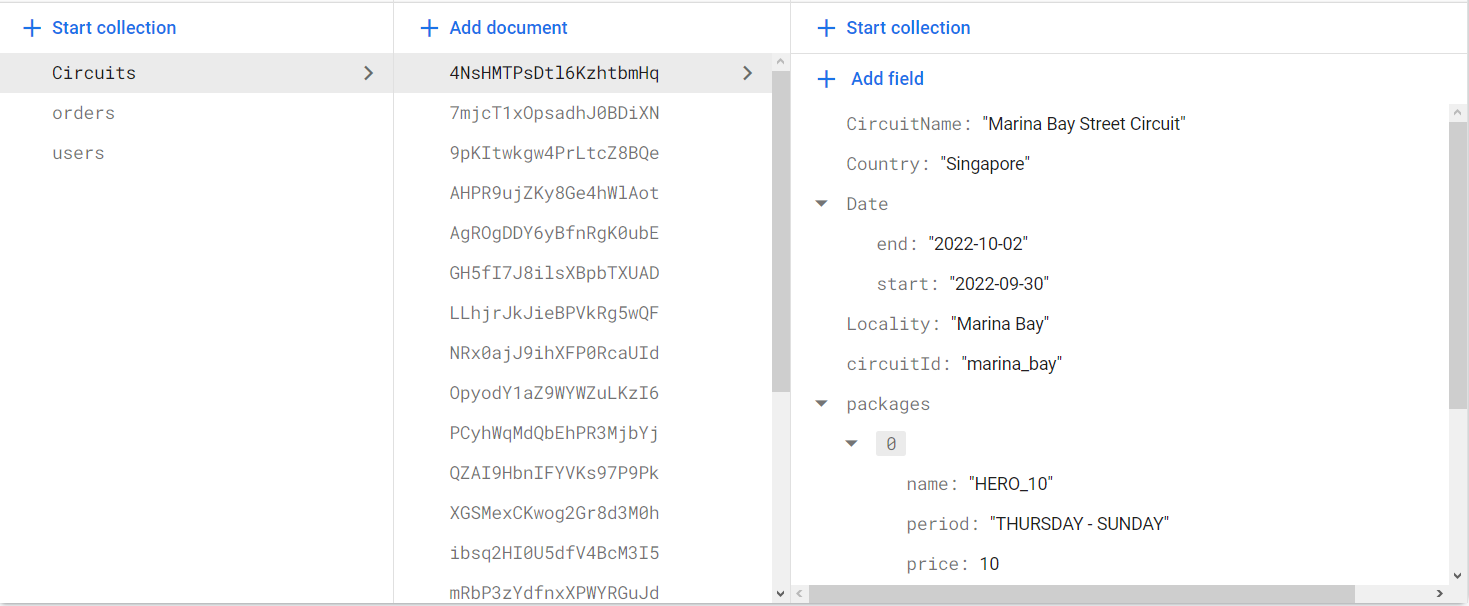
\includegraphics[scale=0.4]{images/firestoreStructure}
	\caption{Cloud Firestore struktúrája}
	\label{abra:firestoreStructure}
\end{figure}

A adatbázis megfelelő biztonságát a \textbf{szabályok} (Rules) beállításával lehet megadni. Ezen szabályok tudják biztosítani, hogy az adott dokumentumokhoz milyen feltételek alapján lehet hozzáférni. Ilyen például, hogy egy felhasználó adataihoz mindig csak a \textit{Firebase Authentication} által bejelentkezett felhasználó férjen hozzá az egyedi azonosító alapján (auth.uid) (\ref{code:databaseRules}).

\begin{lstlisting}[caption={Firestore szabályok.}, captionpos=b, label={code:databaseRules}]
match /databases/{database}/documents {
    match /users/{userId} {
      // Allow users to only read or write their own documents
    	allow read, write: if request.auth.uid == userId;
    }
}
\end{lstlisting}

\subsection {Firebase Storage}

A \textbf{Firebase Storage} szolgáltatás lehetővé teszi a felhasználói fájlok, például képek, videók vagy hangfájlok tárolását és kezelését. A Firebase Storage nagyobb méretű fájlok tárolására és letöltésére specializálódott, amelyeket a Google Cloudban tárolja. Az én alkalmazásomban a feltöltött profilképek kerülnek a Storage-ban tárolásra (\ref{abra:storageStructure}).

\begin{figure}[!h]
	\centering
	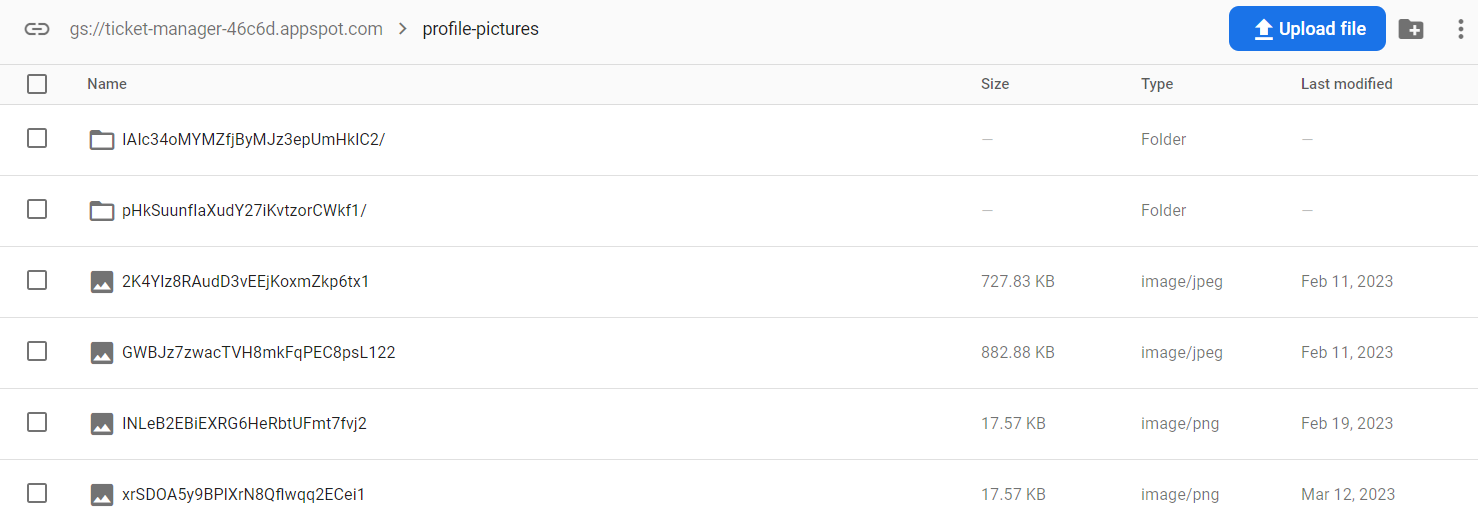
\includegraphics[scale=0.4]{images/storageStructure}
	\caption{Firebase Storage struktúrája}
	\label{abra:storageStructure}
\end{figure}
\pagebreak

\section {Vercel backend architektúra}

A \textbf{Vercel} által kiszolgált egyik backend szerver, amely hasonlóan a frontendhez (\ref{frontend}) JavaScript nyelven van írva \textbf{NodeJS} keretrendszerben (\ref{abra:vercelStructure}). A szerver kiinduló pontja az \textit{app.js}, amely tartalmazza az alapértelmezett konfigurációkat a HTTP hívások kezelésére és a végpontokat tartalmazó fájlok helyét. A szerver textbf{Express} alapú.

A Vercel-en több sablon alapján lehet szervert létrehozni. Én egy egy third-party repository segítségével hoztam létre, amely megtalálható a GitHubon a \textbf{geshan} nevű felhasználó jóvoltából \cite{GitNodeSql}.

Az Express.js, vagy egyszerűen csak Express, egy backend webalkalmazás-keretrendszer RESTful API-k létrehozásához a Node.js segítségével, amelyet ingyenes és nyílt forráskódú szoftverként adnak ki az MIT-licenc alatt \cite{WikiExpress}.

\begin{figure}[!h]
	\centering
	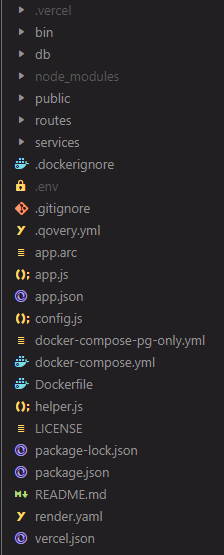
\includegraphics[scale=0.6]{images/vercelStructure}
	\caption{Vercel mappa struktúrája}
	\label{abra:vercelStructure}
\end{figure}

A \textbf{routes} mappa tartalmazza a alkalmazás működéséhez szükséges JSON, CSS és egyéb JS fájlokat. Az én esetemben itt találhatóak az \textit{index.js} és a \textit{quotes.js} fájlok (\ref{abra:vercelRoutes}). Az index.js tartalmazza a szerver végpontjait és az üzleti logikát. A quotes.js pedig a Google Firebase szerverrel való kapcsolat kialakításához szükséges konfigurációkat, amelyek lefutnak a szerver indulásakor.

\begin{figure}[!h]
	\centering
	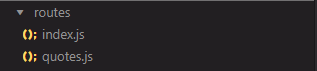
\includegraphics[scale=0.8]{images/vercelRoutes}
	\caption{Vercel \textit{Routes} mappa}
	\label{abra:vercelRoutes}
\end{figure}

A titkosítási és kulcscsere algoritmusok használatára rendre a \textbf{crypto-js} és \textbf{node-rsa} JavaScript könyvtárcsomagokat használom \cite{NRSA} \cite{CJS}. A node-rsa egy optimális és kényelmes használatot nyújt az RSA publikus kulcscsere protokoll beépítéséhez a rendszerbe. Ez egy emelt szintű biztonságot biztosít a felhasználók számára. Azt is figyelembe vettem, hogy ez a kulcscsere csak akkor biztonságos, ha a kulcsokat is biztonságos módon tároljuk. Erre azt a megoldást alkalmaztam, hogy a publikus és privát kulcsokat is a Google Firestore-ban tárolom, amelyre olyan szabályok (rules) vannak beállítva, hogy mindig csak az adott autentikált felhasználó férjen hozzá, ahogyan arról már említést tettem a \ref{firebase} fejezetben a \ref{code:databaseRules} kódrészlet segítségével.